% generated by scripts/pkl_to_latex.py
% source PKL : tscan_v1_L6_Ne6_U10_mode-uniform_nmin2_solver-gcg_full_es_restarts8_iter300_kmax2_tol1em09_t0.05to2_N20-d03538a42051.pkl
% scan type  : tscan
% state      : ex_singlet
% requires   : \usepackage{pgfplots} \pgfplotsset{compat=1.18}
% colours match the matplotlib PDF (tab10 cycle)
\definecolor{gmeC0}{HTML}{1F77B4}
\definecolor{gmeC1}{HTML}{FF7F0E}
\definecolor{gmeC2}{HTML}{2CA02C}
\definecolor{gmeC3}{HTML}{D62728}
\definecolor{gmeC4}{HTML}{9467BD}
\definecolor{gmeC5}{HTML}{8C564B}
\definecolor{gmeC6}{HTML}{E377C2}
\definecolor{gmeC7}{HTML}{17BECF}

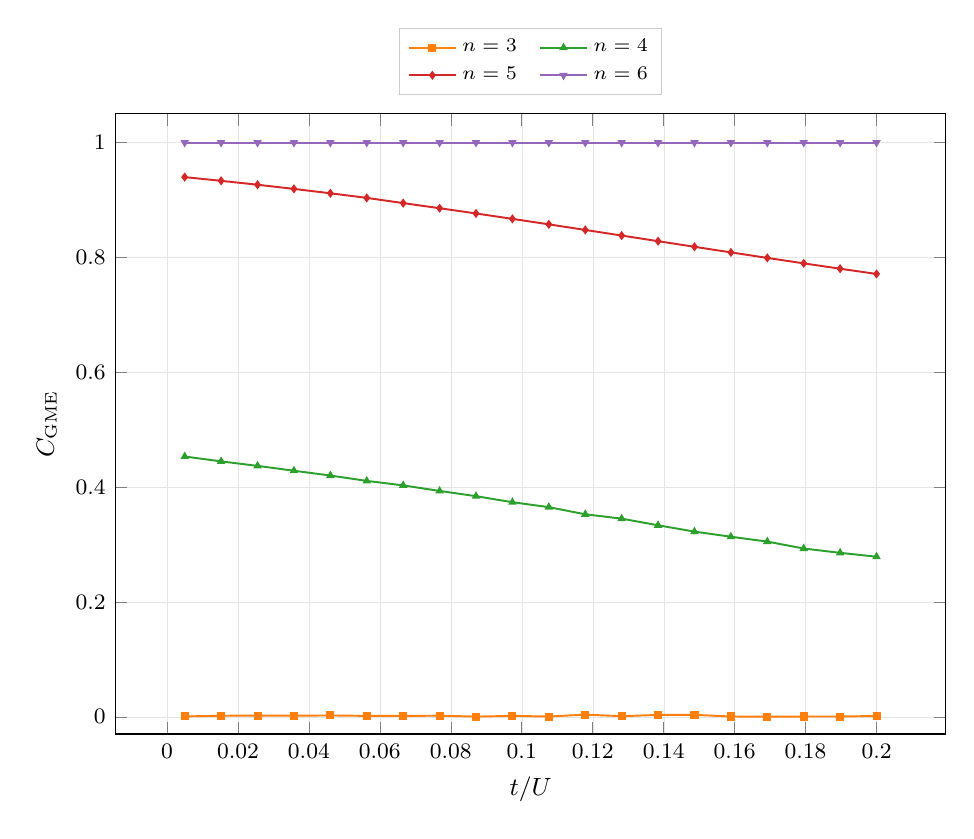
\begin{tikzpicture}
  \begin{axis}[
    width=\columnwidth,
    height=0.78\columnwidth,
    xlabel={$t/U$},
    ylabel={$C_{\mathrm{GME}}$},
    grid=both,
    grid style={line width=.1pt, draw=gray!20},
    tick label style={font=\footnotesize\rmfamily, /pgf/number format/fixed},
    label style={font=\small\rmfamily},
    scaled ticks=false,
    legend style={font=\scriptsize\rmfamily, draw=gray!40, at={(0.5,1.03)}, anchor=south, /tikz/every even column/.append style={column sep=6pt}},
    legend cell align={left},
    legend columns=2,
    ymin=-0.03,
    ymax=1.05,
  ]
    \addplot[color=gmeC1, mark=square*, mark size=1.1pt, line width=0.7pt] coordinates {
        (0.005,0.000691) (0.015263,0.001794) (0.025526,0.002202) (0.035789,0.001914)
        (0.046053,0.002386) (0.056316,0.001597) (0.066579,0.001473) (0.076842,0.001999)
        (0.087105,0.000335) (0.097368,0.001614) (0.107632,0.000475) (0.117895,0.003823)
        (0.128158,0.001037) (0.138421,0.003329) (0.148684,0.003388) (0.158947,0.000548)
        (0.169211,0.000247) (0.179474,0.000516) (0.189737,0.000478) (0.2,0.001458)
    };
    \addlegendentry{$n=3$}
    \addplot[color=gmeC2, mark=triangle*, mark size=1.1pt, line width=0.7pt] coordinates {
        (0.005,0.453315) (0.015263,0.4448) (0.025526,0.436959) (0.035789,0.428496)
        (0.046053,0.420177) (0.056316,0.410821) (0.066579,0.403028) (0.076842,0.393319)
        (0.087105,0.384231) (0.097368,0.373712) (0.107632,0.365102) (0.117895,0.352682)
        (0.128158,0.345069) (0.138421,0.33352) (0.148684,0.322474) (0.158947,0.313603)
        (0.169211,0.305123) (0.179474,0.293067) (0.189737,0.285554) (0.2,0.278791)
    };
    \addlegendentry{$n=4$}
    \addplot[color=gmeC3, mark=diamond*, mark size=1.1pt, line width=0.7pt] coordinates {
        (0.005,0.939829) (0.015263,0.933401) (0.025526,0.926557) (0.035789,0.919308)
        (0.046053,0.911673) (0.056316,0.903671) (0.066579,0.89457) (0.076842,0.885698)
        (0.087105,0.876543) (0.097368,0.867152) (0.107632,0.857578) (0.117895,0.847874)
        (0.128158,0.838091) (0.138421,0.828281) (0.148684,0.81849) (0.158947,0.808762)
        (0.169211,0.799136) (0.179474,0.789645) (0.189737,0.780317) (0.2,0.771176)
    };
    \addlegendentry{$n=5$}
    \addplot[color=gmeC4, mark=triangle*, mark size=1.1pt, mark options={rotate=180}, line width=0.7pt] coordinates {
        (0.005,1) (0.015263,1) (0.025526,1) (0.035789,1)
        (0.046053,1) (0.056316,1) (0.066579,1) (0.076842,1)
        (0.087105,1) (0.097368,1) (0.107632,1) (0.117895,1)
        (0.128158,1) (0.138421,1) (0.148684,1) (0.158947,1)
        (0.169211,1) (0.179474,1) (0.189737,1) (0.2,1)
    };
    \addlegendentry{$n=6$}
  \end{axis}
\end{tikzpicture}
